%%*****************************************************************************
%% $Id$
%%*****************************************************************************
%% @author Gerd Neugebauer
%%-----------------------------------------------------------------------------
\chapter{Source Code Documentation}


The source code has to be documented. \TeX\ shows us a good example of
a proper documenatation. Donald Knuth has invented the Web system to
keep together the documentation and the source code. The source code
and documentation are extracted from a common file. In the Java world
the Javadoc system has been invented for a similar purpose. 

\section{Javadoc}

The Javadoc conventions for comments make it possible to extract the
relevant part of the documentation and generate several outut formats
from it. The primary output format is HTML.
\begin{figure}[tbh]
  \centering
  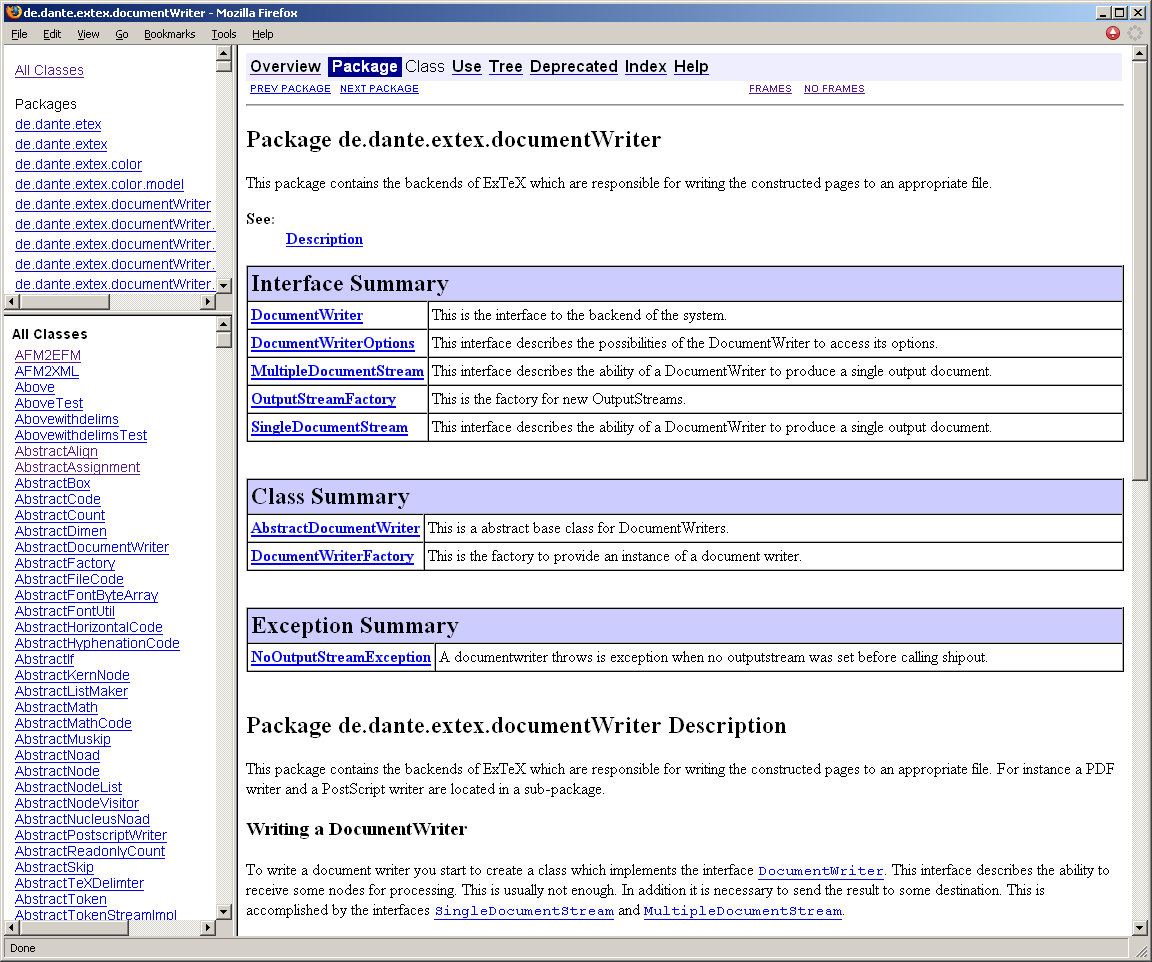
\includegraphics[scale=.33]{image/javadoc}
  \caption{Javadoc in the Browser}\label{fig:eclipse-javadoc}
\end{figure}

\section{Documentation of Primitives}

The documentation of the primitives is contained in the Javadoc
comments of the implementing Java classes. A script is used to extract
the information from the sources for the User's Manual. To make this
happen, the documentation meant for the manual has to be marked and
formatted specially.

\INCOMPLETE


